\documentclass[statementpaper,oneside,article,14pt]{memoir}
\usepackage{geometry}
\usepackage{libertine}
\usepackage{kantlipsum}

% Disable chapter/section numbering.
\setsecnumdepth{none}
\maxsecnumdepth{none}

% Optional background
% http://tex.stackexchange.com/a/276280
\usepackage{tikz}
\usepackage{tikz-network}
\usepackage{transparent}
\usepackage{eso-pic}
\usepackage{listings}
\usepackage{xcolor}
\usepackage{sourcecodepro}
\usepackage[T1]{fontenc}

\newcommand{\BackgroundPic}[1]{%
\put(0,0){%
\parbox[b][\paperheight]{\paperwidth}{%
\vfill
\centering
{\transparent{0.4} \includegraphics[width=\paperwidth,height=\paperheight,%
keepaspectratio]{#1}}%
\vfill
}}}

\definecolor{codegreen}{rgb}{0,0.6,0}
\definecolor{codegray}{rgb}{0.5,0.5,0.5}
\definecolor{codepurple}{rgb}{0.58,0,0.82}
\definecolor{backcolour}{rgb}{0.95,0.95,0.92}

% \lstset{basicstyle=\ttfamily}

\lstdefinestyle{mystyle}{
    backgroundcolor=\color{backcolour},   
    commentstyle=\color{codegreen},
    keywordstyle=\color{magenta},
    numberstyle=\tiny\color{codegray},
    stringstyle=\color{codepurple},
    basicstyle=\ttfamily\footnotesize,
    breakatwhitespace=false,         
    breaklines=true,                 
    captionpos=b,                    
    keepspaces=true,                 
    numbers=left,                    
    numbersep=5pt,                  
    showspaces=false,                
    showstringspaces=false,
    showtabs=false,                  
    tabsize=2
}

\lstset{style=mystyle}

\begin{document}

% Edit inside the { brackets } to change these.

\title{Modelling Computation as Tensors}
\author{Nimalan M}
\date{Nov 23}

\begingroup
\let\cleardoublepage\clearpage

% \AddToShipoutPicture*{\BackgroundPic{samplecover}}

\begin{titlingpage}
\maketitle

% Could add a small author's note, etc. here if you like.

\end{titlingpage}

\endgroup

% As the zine is so short, you probably won't need page numbers; however, if you
% want them, comment out the next line with a %.
\pagestyle{empty}


%% CONTENT GOES BELOW


\section{Linear Algebra and Tensors}

Tensors are a more nature way to representing computational problems which are derived from Linear Algebra. Modelling computations as tensors saves the scientist a lot of effort in programming and allows them to focus more on the problem they are solving.

Let us consider for this case that a tensor is a multidimensional arrary. A rank zero tensor is a scalar, rank-1 tensor is a vector and rank-2 tensor is a matrix. A tensor contraction is the summation over all values of indices of a set of tensors.

For example matrix multiplication can be represented in the Einstein notation or index notation as

$$ C_{ij} = A_{ik} B_{kj}  $$

or in the Penrose graph notation as

\begin{center}
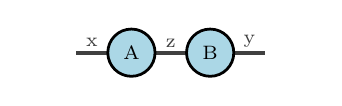
\begin{tikzpicture}
  \Vertex[x=0,Pseudo]{A'}
  \Vertex[x=1,IdAsLabel]{A}
  \Vertex[x=2,IdAsLabel]{B}
  \Vertex[x=3,Pseudo]{B'}
  \Edge[label=x,position=above](A')(A)
  \Edge[label=z,position=above](A)(B)
  \Edge[label=y,position=above](B)(B')
\end{tikzpicture}
\end{center}

\newpage
\section{Computation of Tensors}

A lot of libraries these days allow working with tensors. Examples in Python numpy, cupy, jax, etc and even machine learning libraries like tensorflow and pytorch. In C++ there is xtensor, MatX etc.

\vfill

\begin{lstlisting}[language=Python]
import numpy as np

a = np.randn(2, 5)
b = np.randn(5, 4)

# Matrix multiplication
c = a @ b

l = np.randn(2, 3, 4)
m = np.randn(3, 4, 5)
n = np.randn(2, 3, 5)

# Tensor reduction
np.einsum("ijk,jkx,ijx->ij", l, m, n)
\end{lstlisting}

\newpage
\section{Composing Transforms}

The true benefit of modelling computations as tensors arise when we chose libraries that allow for composing transforms on tensors.

\vfill

\begin{lstlisting}[language=Python]
import jax.numpy as np
from jax import jit

@jit
def fn(B, C, D):
  return (B * cos(C)) / D

@jit
def fn2(A, B, C):
  D = jnp.einsum("ijk,ij->ij", A, C)
  E = jnp.einsum("ijk,ij->ij", B, C)
  return jnp.stack([D, E])
\end{lstlisting}

\vfill

In the above example the \texttt{@jit} tag, performs a JIT compilation and composed the transformations. Depending on the nature of the library even more complex transformations can be composed.

\newpage
\section{Tensor Decomposition}

\vfill

\begin{center}
  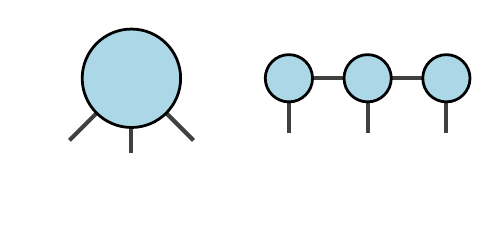
\begin{tikzpicture}
    \Vertex[size=1.25]{R}
    \Vertex[x=-1,y=-1,Pseudo]{R'}
    \Vertex[x=0,y=-1.25,Pseudo]{R''}
    \Vertex[x=1,y=-1,Pseudo]{R'''}
    \Edge(R)(R')
    \Edge(R)(R'')
    \Edge(R)(R''')
    
    \Vertex[x=2]{A}
    \Vertex[x=3]{B}
    \Vertex[x=4]{C}
    \Vertex[x=2,y=-1,Pseudo]{A'}
    \Vertex[x=3,y=-1,Pseudo]{B'}
    \Vertex[x=4,y=-1,Pseudo]{C'}
    \Edge(A)(A')
    \Edge(B)(B')
    \Edge(C)(C')
    \Edge(A)(B)
    \Edge(B)(C)
  \end{tikzpicture}
\end{center}

\vfill

Another technique for computing tensors in hardware is to decompose higher order tensors into multiple smaller order tensors. These smaller order tensors are then batched and processed in parallel in hardware.

\vfill

\begin{lstlisting}[language=Python]
import jax.numpy as jnp

#  ([a], [a]) -> []
vv = lambda x, y: jnp.vdot(x, y) 

#  ([b,a], [a]) -> [b]
mv = vmap(vv, (0, None), 0)

#  ([b,a], [a,c]) -> [b,c]
mm = vmap(mv, (None, 1), 1)
\end{lstlisting}

\vfill

The above is an example of starting with a order 1 tensor operation vector dot product and deriving matrix multiplication

\vfill

\newpage
\section{Hardware Acceleration}

\vfill

A lot of modern hardware accelerators have dedicated tensor processors/core to accelerate tensor operations.

GPUs with tensor cores usually have better performance when working with tensors.

jax uses LLVM's MLIR to target GPUs and Google TPUs.

\vfill

\begin{figure}[htp]
  \centering
  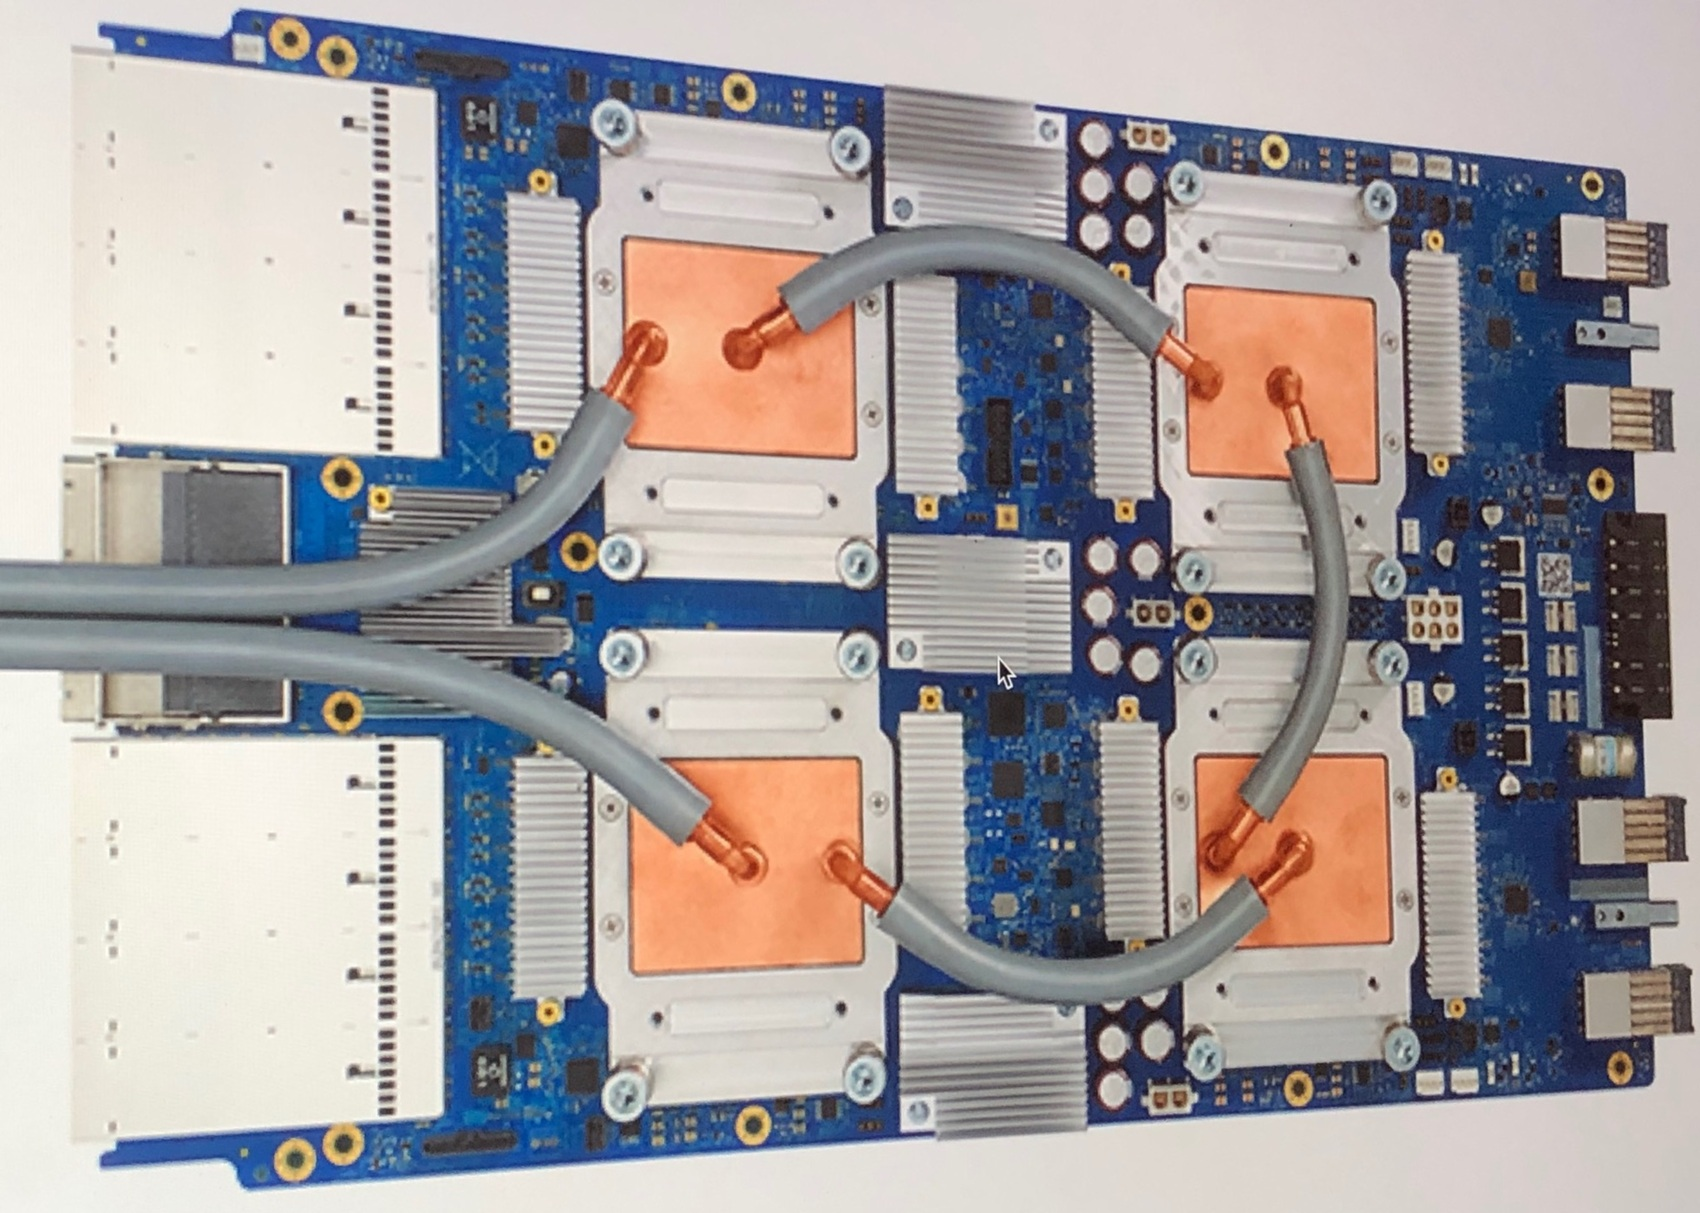
\includegraphics[width=10cm]{TPU}
  \caption{Google TPU 3.0}
  \label{fig:tpu}
\end{figure}

\vfill

% Tensor Network diagrams can also be interpreted as Category Theory string diagrams. Tensors form a category. The Vec category has vector spaces as objects and linear maps between vector spaces are morphisms.

\newpage
\section{Tensors and Category Theory}

Tensors form a category. The Vec category has vector spaces as objects and linear maps between vector spaces are morphisms. As an example let $M: A \to B$, $N: B \otimes C \to D$, $P: D \to E$ be linear maps between finite vector spaces $A, B, C, D, E$. These can be combined to obtain $F: A \otimes C \to E$, or this can be written as

$$
F = P \circ N \circ (M \otimes id_c)
$$

In the mathematical notation this is

$$
f_{m_ik} = \sum_j \sum_l p_{m,l} n_{l,jk} m_{j,i}
$$

In the einstein notation this is

$$
F_m^{ik} = P_m^l N_l^{jk} M_j^i
$$

And in the penrose graphical notation

\begin{center}
  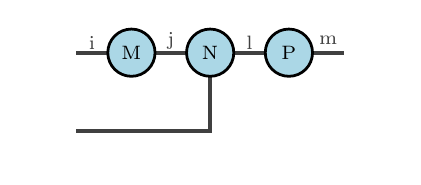
\begin{tikzpicture}
    \Vertex[x=-1,y=-1,Pseudo]{K'}
    \Vertex[x=-1,y=0,Pseudo]{I'}
    \Vertex[x=0,y=0,IdAsLabel]{M}
    \Vertex[x=1,IdAsLabel]{N}
    \Vertex[x=2,IdAsLabel]{P}
    \Vertex[x=3,Pseudo]{M'}
    \Edge[path={K',{1,-1},N},label=k,position=above](K')(N)
    \Edge[label=i,position=above](I')(M)
    \Edge[label=j,position=above](M)(N)
    \Edge[label=l,position=above](N)(P)
    \Edge[label=m,position=above](P)(M')
  \end{tikzpicture}
\end{center}

%% CONTENT ENDS

% Back cover

\newpage

\centering

\section{}

\vfill

By Nimalan M \\
Github - (@mark1626) \\

Licensed under Creative Commons BY

\begin{figure}[htp]
  \centering
  
\includegraphics[width=4cm]{cc_by}
  \label{fig:cc}
\end{figure}

\vfill

\end{document}
